\documentclass[12pt]{article}
\usepackage{mandi}
\usepackage{braket}
\usepackage{graphicsx}
\usepackage{amsmath}
\usepackage{amsfonts}
\tolerance=1
\emergencystretch=\maxdimen
\hyphenpenalty=10000
\hbadness=10000
% Palatino font (ppl must be installed).
%\renewcommand*\rmdefault{ppl}
% Iwona font (iwona must be installed).
%\renewcommand*\rmdefault{iwona}
\begin{document}
\title{Quantum Algorithms: A Survey}
\author{Anurag Pallaprolu \\ Physics and Electronics \\ BITS Pilani \\ Rajasthan}
\maketitle
\begin{abstract}
The present document deals with a few of the famous algorithms used in quantum computation and quantum searching. It mainly discusses the \textbf{Deutsch Algorithm, Deutsch Josza Algorithm, Grover's Algorithm and Shor's factoring algorithm} in simple details. The document exemplifies the advantages of quantum mechanical construction of computational and information processing devices and also deals with \textbf{quantum parallelism}, the one feature that leads to the multiplication of computing power.
\end{abstract}

\section{Wait, What is quantum doing in computer science?}
This is a very common question that pesters many  beginning computer science and physics students alike, like me. Personally, when I started reading quantum, I never saw any practical use for the science and I always thought that it was a subject only useful in particle physics and solid state electronics. This document is my condensation of the implementation of this unwieldy approach in computer science. The main idea behind any parallel computational approaches other than the traditional voltage level paradigm is that, \textbf{any two state system with distinguished boundaries for each state can be used as a 0 and a 1 in computation.} Luckily for us, most of the computation is based on \textit{Boolean} logic and hence can be adapted to any sort of two state system. This is the heart of quantum computation. Biological techniques are used to analyze computing methods involving the coding on a DNA helix, the genetic pairing of chromosomes etc., and these can be translated into parallel Boolean languages, and the branch is commonly referred to as Bioinformatics. In this case, the spin of an electron, the dipole moment of $NH_3$ molecule can all be used as two state systems and are analyzed using quantum mechanical techniques such as the \textbf{density operator} formulation due to John von Neumann or the unitary \textbf{matrix mechanics} due to Werner Heisenberg and Pascual Jordan. Just as in traditional computers(processors) digital devices or \textbf{gates} are used to represent a given logic blueprint, quantum computers also consist of \textbf{quantum gates}. Here is where the intersection takes place and this is the right place to start.

\section{A Quick and Dirty Introduction to Quantum Computing Terminologies}
\subsection{Qubit}
I shall start out by explaining what a quantum bit or a \textbf{qubit} is. The name is self explanatory. Let me just point out the crucial difference, a classical bit can, at any point of time, take only one of the two quantized boolean states. Quantum bits on the other hand can be in a simultaneous superposition state of the individual quantized values. To put it symbolically,
\begin{center}
IN CLASSICAL COMPUTATION
\end{center}
$$\Ket{0}, \Ket{1}$$
\begin{center}
IN QUANTUM COMPUTATION
\end{center}
$$\frac{\Ket{0}+\Ket{1}}{\sqrt{2}}$$
 The $\sqrt{2}$ factor is completely arbitrary. In general, the two ket states might have any arbitrary (normalized) amplitudes. The behavior of these states is governed by the laws of quantum mechanics. That's all there is for a qubit. Now let us look at a few operations on qubits. They exist in vector spaces(more on this later) and can be operated on any two vectors. They could also be operated on each other using any standard vector arithmetic. An inner product can be established on the vector space in which the kets exist(more on this later).  The first question that might occur to any opportunistic person would be to expand this amalgamated state to more than one bit. This can be done due to the wonderful mathematical process of taking the \textbf{tensor product} or the \textbf{Kronecker product} of two or more qubits. The idea is quite simple and is exactly like the \textbf{direct product of two sets}. 
$$\frac{\Ket{0}+\Ket{1}}{\sqrt{2}}\otimes\frac{\Ket{0}-\Ket{1}}{\sqrt{2}} = \frac{1}{\sqrt{2}}(\Ket{00}-\Ket{01}+\Ket{10}-\Ket{11})$$
Your first thought might be, what in the world is $$\Ket{00}$$Well, don't get bewildered. Just think of it as a larger ket vector tracing two smaller qubit ket components. Let us talk about quantum gates to make this concept clear. 
\subsection{Quantum Gate}
A \textbf{gate} in any device is in general a logical unit which operates on Boolean variables. A \textbf{quantum gate} is a device which operates on \textit{quantum} boolean variables. I have to state a few facts before going into the explanation of the workings of a quantum gate. Every quantum mechanical operation takes one ket from the \textbf{Hilbert Space} in which it exists to another one with the help of a (matrix) transformation called as a \textbf{unitary transformation}. You might have heard of unitary matrices. Well, according to linear algebra, any linear transformation on a vector can be represented by a \textbf{matrix of transformation}. If this matrix turns out to be unitary, a situation which is most favorable for representing changes in quantum ket states, then it is a unitary transformation. This is a very bare bones version of one of the postulates of quantum mechanics. For a fuller explanation, refer to any standard quantum text like \textit{Griffiths}, \textit{Sakurai} or \textit{Shankar}. Anyway, any operation on a ket can be seen as a unitary matrix operating on its vector representation. Now, gates also operate on kets/qubits. Hence, the moral of the above story is that \textbf{every quantum gate can be represented in its unitary matrix representation}. For example, look at the simple circuit next page,\\
\begin{center}
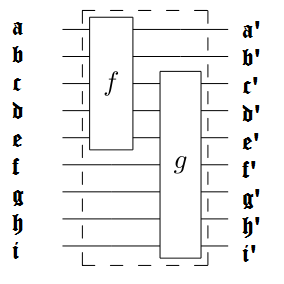
\includegraphics[scale=0.8]{qgate1.png}
\end{center}
The input lines all carry one qubit each. The gate $f$ operates on the first five lines and then the $g$ gate operates on the last seven lines. The input can be seen as a tensor product multi-qubit of 9 single qubits represented compactly as
$$\Ket{\Psi} = \bigotimes_{x=a}^{x=i}\Ket{x}$$ For instance, if each of the inputs was $\Ket{0}$, then $\Ket{\Psi} = \bigotimes_{x=a=0}^{x=i=0}\Ket{0}=\Ket{000000000}$. As discussed before, \textit{the operation of the $f$ gate can be represented by a unitary transformation on the initial (multi)ket}. Let us call this matrix as $\mathcal{F}$. Then the next state of the combined qubit after the $\mathcal{F}$  would then be $$\mathcal{F}\bigotimes_{x=f,x'=a}^{x=i,x'=e}\Ket{x'}\Ket{x} = \bigotimes_{x=f,x'=a}^{x=i,x'=e}\mathcal{F}\Ket{x'}\Ket{x}$$ Note the change in the indices of summation as not all individual qubits are going through $\mathcal{F}$. Let's call the multiqubit at this step as $\Ket{\Psi_{1}}$.The next step would be to operate $g$ onto the qubits $c$ through $i$. Let's call its matrix as $\mathcal{G}$. The qubit at this stage would be $$\mathcal{G}\Ket{\Psi_{1}} =  \bigotimes_{x=f,x'=a}^{x=i,x'=e}\mathcal{F}\Ket{x'}\mathcal{G}\Ket{x}$$
$$\bigotimes_{x=f,x'=a}^{x=i,x'=e}\mathcal{F}\Ket{x'}\mathcal{G}\Ket{x} = \bigotimes_{x=a'}^{x=i'}\Ket{x}$$
The concept of parallelism should get a bit clear now as you can clearly see the individual operation of gates on qubit, but the final (unnormalized) state is correlated. This should also point out one of the major issues with parallelism theory, \textit{we can compute a state in \textbf{one} step which contains, say, the values of the function $f(x)$ for many values of $x$(whereas a classical computer would take $n$ steps where $n$ is the number of values of $x$). But to access the values, we have to perform a measurement, and a measurement performed on a particular $\Ket{x}$ would lead to the \textbf{collapse of the ket at the value}}. The last line quantum mechanically tells us that we would lose information about all other values of $x$  but retain the value of $f(x_{measured})$. This might sound like quantum computing just lost a point against its classical opponent, but where it wins is (as we shall see in Deutsch's Algorithm next) the final state can be a combination of operated individual values, like $f(x_1)+f(x_2)$ etc., which the classical computer \textbf{would still take $n$ steps to do(in the present case 2)}. You can read up more on standard quantum gates from \textit{Nielson and Chuang}, but I think this discussion shall suffice for the documentation.
\subsection{Walsh-Hadamard Transform}
However, I shall describe one specific type of gate, called the \textbf{Hadamard Gate} named after Jacques Hadamard. It is represented by the symbol 
\begin{center}
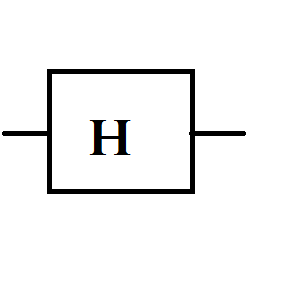
\includegraphics[scale=0.5]{qhad.png}
\end{center}
Simply put, let us take any qubit in the standard basis of $\mathbb{H}$ say $\Ket{\psi} = \alpha\Ket{0} + \beta\Ket{1}$. The operation of $\mathcal{H}$ on standard basis qubits is known $$\mathcal{H}\Ket{0} = \frac{\Ket{0}+\Ket{1}}{\sqrt{2}}$$
$$\mathcal{H}\Ket{1} = \frac{\Ket{0}-\Ket{1}}{\sqrt{2}}$$
With this, now we can see
$$\mathcal{H}\Ket{\psi} = \alpha\frac{\Ket{0}+\Ket{1}}{\sqrt{2}} + \beta\frac{\Ket{0}-\Ket{1}}{\sqrt{2}} = \frac{\alpha + \beta}{\sqrt{2}}\Ket{0} + \frac{\alpha - \beta}{\sqrt{2}}\Ket{1}$$
Hence, as you can see, the operation is quite simple, and one can easily derive the transformation matrix of $\mathcal{H}$. Now, let us take two qubits, for simplicity, let both of them be $\Ket{0}$. Now, let us apply the \textbf{Hadamard Gate on 2 Qubits or the Nth order Hadamard Gate} represented by $\mathcal{H}^{\bigotimes 2}$. This is nothing but the operator $\mathcal{H}\bigotimes\mathcal{H}$. Thus, two Hadamard gates operate on individual qubits and are again \textit{tensorially} combined into one qubit. Note the pattern of $\mathcal{H}^{\bigotimes n}$ as $n$ increases, as given below.
$$\mathcal{H}^{\bigotimes 2}\Ket{00} = \mathcal{H}\Ket{0}\mathcal{H}\Ket{0} = \frac{\Ket{00}+\Ket{01}+\Ket{10}+\Ket{11}}{2}$$
$$\mathcal{H}^{\bigotimes 3}\Ket{000} = \frac{\Ket{000}+\Ket{001}+....+\Ket{101}+\Ket{111}}{2^{3/2}}$$ Notice how all the binary numbers upto $2^n$ are being listed in the combined multikets. This general Hadamard Transform of $n$ qubits can be combined mathematically as
$$\mathcal{H}^{\bigotimes n}\Ket{0^n} = \sum_{x=0}^{x=2^n-1}\frac{\Ket{x}}{\sqrt{2^n}}$$ This operation is much more generally known as the \textbf{Walsh-Hadamard Transform} and comes under a general class of such summable or integrable transforms known as \textit{Fourier Transforms} but we shall not go into this much deep. We have assembled all tools needed to discuss quantum algorithm logic design and we shall head straight to
\section{Deustch's Algorithm}

\end{document}